%卒論概要テンプレート ver. 3.0

\documentclass[uplatex,twocolumn,dvipdfmx]{jsarticle}
\usepackage[top=22mm,bottom=22mm,left=22mm,right=22mm]{geometry}
\setlength{\columnsep}{10mm}
\usepackage[T1]{fontenc}
\usepackage{txfonts}
\usepackage[expert,deluxe]{otf}
\usepackage[dvipdfmx,hiresbb]{graphicx}
\usepackage[dvipdfmx]{hyperref}
\usepackage{pxjahyper}
\usepackage{secdot}





%タイトルと学生番号,名前だけ編集すること
\title{\vspace{-5mm}\fontsize{14pt}{0pt}\selectfont 継続的インテグレーションを用いた文書検査システムの構築}
\author{\normalsize プロジェクトマネジメントコース 矢吹研究室 1342097 浜野太豪}
\date{}
\pagestyle{empty}
\begin{document}
\fontsize{10.5pt}{\baselineskip}\selectfont
\maketitle





%以下が本文
\section{序論}



\noindent

ドキュメントの検査にプログラムやツールによるサポートが必要である.なぜなら,システム開発の現場では,様々なドキュメントを作成する必要があるからだ.例えばプロジェクト計画書や要件定義書,マニュアルなどがある.このような文書では,読み手に誤解を与えてはいけない.さらに,わかりやすい文書を書くには一定のルールを守る必要がある.短い文で書くこと,正しい表現方法で書くこと,フォーマットを統一することなどである.このようなルールで,大量のドキュメントを人の目によってチェックすることには限界がある.

そこで継続的インテグレーションを活用する方法がある.継続的インテグレーションとは,プログラム全体を常に統合して動く状態にしておくことである.最近では,ビルド(プログラムのコンパイルや自動テスト,アーカイブ化,ソースコードへのタグ付け,実行環境へのデプロイの一連の手順)を自動化するツールが数多くある\cite{1}.

このような継続的インテグレーションで活用されている自動化ツールを用いて,大量のドキュメントをチェックできるツールを構築する.








 



\noindent


\section{目的}
文書チェックを自動的に行うシステムを構築する.
研究室ではドキュメントの変更履歴をバージョン管理システムGitHubを用いて管理している.GitHubに文書を提出した際に,自動で文書チェックプログラムが実行され,実行結果の表示,通知を行う.

\section{手法}
構築の手法について以下に示す.
\begin{enumerate}
\item 文書チェックプログラムの設定を行う.
\item 自動化ツールの設定を行う.
\item 文章チェックプログラムと自動化ツールとGitHubの連携を行う.
\end{enumerate}

\section{結果}
GitHubに課題研究の概要を提出した場合,文章チェックプログラムによって自動的に文章チェックが行えるようになった.
課題研究の概要を文書チェックにかけてみたところ以下の指摘が表示された.
\begin{enumerate}
\item SentenceLength - 文長を検査する.
\item InvalidExpression - 不正な表現が利用されていないか検査する.
\item KatakanaSpellCheck - カタカナ単語のスペルチェックを行う.
\item JapaneseAmbiguousNounConjunction - 助詞の「の」が連続しているか検査する.
\end{enumerate}
\begin{figure}[htb]
\centering 
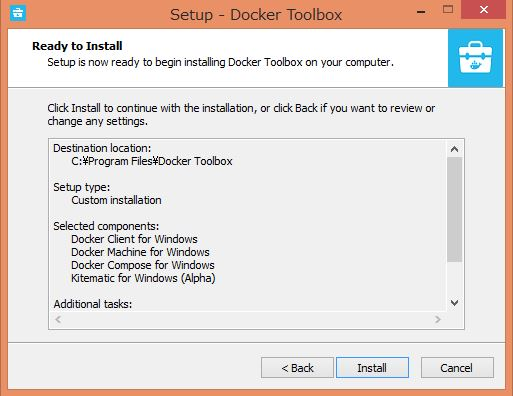
\includegraphics[width=6cm]{7.JPG}
\caption{文書チェック結果}
\end{figure}


\section{考察}

文書チェックプログラムは設定ファイルを変更することで,出力結果も変わる.そのため設定を変更し,添削に有効な設定を検討する必要がある.例えば添削前の文書を文書チェックプログラムにかけ,どの範囲まで文書の誤りをチェックすることができるのか調べることで,文書チェックプログラムが添削できる範囲を調べることができると考えた.

\section{結論}
自動的に文書チェックを行う環境を構築することができた.文書チェックプログラムの設定に関しては詳しく調べることができなかったため,検証が必要である.


\bibliographystyle{junsrt}
\bibliography{biblio}%「biblio.bib」というファイルが必要.

\end{document}
